\chapter{Dark matter: beyond the Standard Model}
\label{chap:DM}
%% Restart the numbering to make sure that this is definitely page #1!
\pagenumbering{arabic}

The Standard Model (SM) of particle physics, albeit a successful theory encoding the properties of elementary particles and their interactions, nonetheless has some shortcomings. For one, cosmological and astrophysical observations supply compelling evidence~\cite{Bertone:2004pz, Feng:2010gw, Porter:2011nv} for the existence of dark matter (DM), a piece of the astro-particle physics puzzle that is not covered by the SM. In \SectionRef{sec:DMintro}, evidence of the existence of DM and motivations for its search are briefly detailed. Subsequently, an outline of the SM is presented in \SectionRef{sec:SM}, in order to provide context for the prevalent DM candidates described in \SectionRef{sec:DMcandidates}, while in \SectionRef{sec:DMsearches} the three main modes of DM detection are outlined, with a particular emphasis on particle colliders. The chapter concludes with a focus on beyond the Standard Model (BSM) simplified models of DM currently being probed at general-purpose detectors at the Large Hadron Collider (LHC) in Geneva, Switzerland.

\section{Introduction to dark matter}
\label{sec:DMintro}

Observations at all scales, from smaller dwarf galaxies to large galactic superclusters point to the existence of more matter than can be reconciled with the amount of visible matter in our universe. The existence of additional non-luminous matter and its dominance in amount compared to luminous matter, was first postulated by Swiss physicist Fritz Zwicky in 1933 during his studies of the Coma cluster. Zwicky's observations pointed to the necessity for approximately 400 times~\cite{2009GReGr} the mass density as observed from the luminous matter from the cluster to ensure the gravitational bounding of nebulae within Coma. It is worth noting that Zwicky's calculations made extensive use of Hubble's constant at the time, H$_0$ = 558 km/s/Mpc, and if rescaled by the modern value of H$_0 = 67.27 \pm 0.66$ km/s/Mpc~\cite{Ade:2015xua} Zwicky's results point to approximately a mass density 10 times larger than observed~\cite{Bertone:2016nfn}. The period around the 1950's and 1960's marks a time when various astronomical explanations for the missing mass in galaxy clusters began to be ruled out, such as the hypothesis that dark matter consists of hot intracluster gas. \cite{MEEKINS1971} presents evidence that the amount of gas required for gravitational binding is $98\%$ larger than that observed from X-ray emission spectra. During the 1970's the first explicit statements began to emerge regarding the need for the missing mass to be concentrated in the outer parts of galaxies based on spectroscopic and radio astronomy observations of the galactic rotation velocity curves. Namely, Kent Ford and Vera Rubin published results from observations of the Andromeda galaxy which extended the observational reach out to 110 minutes of arc away from the center of M31, revealing a flat dependence of $v$, the galactic rotation velocity, as a function of the radius $r$ beyond the visible galactic disk as shown in~\FigureRef{fig:rubin}. The visible matter in M31 would suggest a steady decrease in $v$ as a function of $r$, but the findings reported by Rubin and Kent point to a flat linear dependence, meaning there is a non-luminous contribution of matter accounting for the additional $v$ beyond the visible disk. By the onset of the 1980's the majority of the astrophysical community was convinced that a substantial amount of DM exists in the universe based on the observational evidence of mass-to-light ratios of galaxies and galactic rotation curves.

\begin{figure}
  \centering
  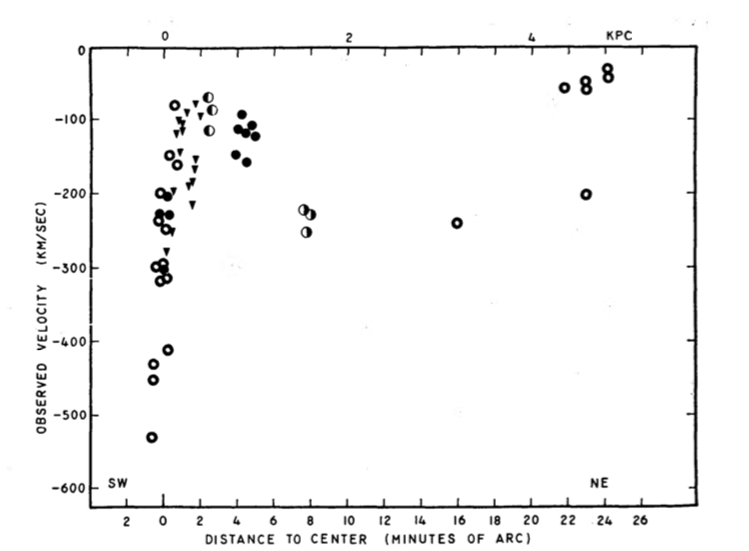
\includegraphics[width=\textwidth]{figs/RubinFordVel}
  \caption{The velocities of emission regions from M31 as a function of distance to the center of the galaxy measured in minutes of arc along the NE major axis as reported by Rubin and Ford in \cite{Rubin:1970zza}.}
\label{fig:rubin}
\end{figure}

Studies of the large scale structure of the universe have provided clues on the nature of dark matter. Just as on the small scale, ordinary visible matter consists of protons, electrons, neutrons, or groups of atoms held together by the electromagnetic force, analogously groups of massive stars and planets were bound together by the gravitational force in order to form stellar clusters. These groups were in turn merged with gas and the postulated DM to form galaxies, and the galaxies were bound together to form clusters, and subsequently superclusters. This standard theory of cosmic structure formation is often referred to as the ``bottom-up'' approach, and essentially posits that the current structure of the Universe is a result of the gravitational amplification of tiny matter fluctuations that were generated during the very early epochs of the Universe~\cite{Allen:2002eu}. The evidence from the 20th century for the existence of non-luminous matter has been further supplemented with data from weak~\cite{Refregier:2003ct} and strong~\cite{Tyson:1998vp} gravitational lensing by large scale structures. The distortion of the appearances of distant objects or the duplication of the apparent image is caused by the bending of the light these objects emit by the gravitational force of the large scale structures in between the observer and the object. The data from a survey of the Bullet cluster as observed by the Chandra~\cite{Markevitch:2005vi} experiment best illustrates how the distribution of the hot gas and stars originating from the collision of two galaxies and comprising the baryonic matter are bound together by a much greater contribution of non-luminous matter as seen in~\FigureRef{fig:bulletcluster}. The calculation of the approximate contribution of visible matter was performed using data from gravitational lensing.

\begin{figure}
  \centering
  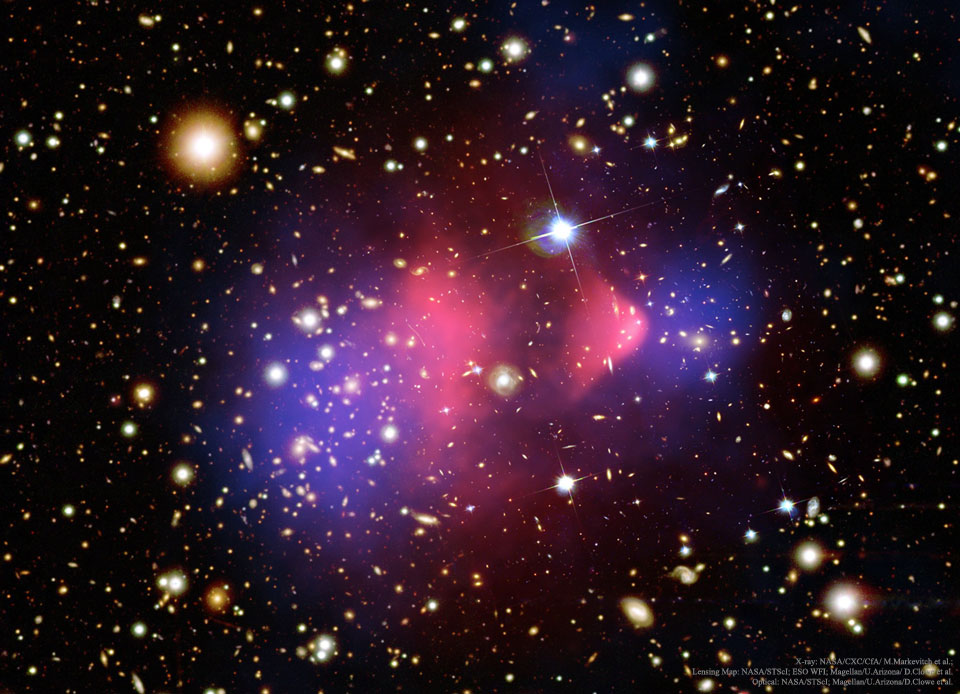
\includegraphics[width=0.8\textwidth]{figs/bulletcluster_comp_960.jpg}
  \caption{A composite image from the Hubble, Chandra, and Magellan telesopes of the 1E 0657-558 cluster of galaxies (Bullet cluster) depicting the X-rays emitted by the baryonic matter as a diffuse red gas, while the approximate location of the DM surrounding the visible matter is represented in a blue hue.}
\label{fig:bulletcluster}
\end{figure}

The aforementioned experiments and measurements buttress the necessity for the existence of DM, however the first attempts to precisely quantify the amount of DM in the Universe began with the discovery and subsequent analyses of the cosmic microwave background (CMB) by Peebles, Wilkinson, Dicke, and Roll~\cite{Dicke1965}. In brief, the CMB is the relic radiation energy content from beyond our galaxy, emitted shortly before the period of recombination~\cite{Seager:1999km} which occured approximately 380 000 years after the Big Bang. At this stage, photons began to decouple from the baryonic matter and over time have been redshifted to the microwave frequency range as a result of the expansion of the Universe over the past 13.81 billion years. Although the dominant contributions of the CMB are homogeneous and isotropic wherein the CMB temperature is almost uniformly $T\simeq2.72\:\mathrm{K}$, slight temperature fluctuations of $\mathcal{O}(10^{-5})$ have been observed which are indicative of the state of the early Universe and the relative abundance of visible and dark matter during this period. As gravity acted on the photon-baryon plasma, the fluid pressure increased giving way to its expansion. This cycle was repeated once the pressure decreased as a result of the expansion, and gravity once more won over causing a fluid compression, hence the photons emitted during different compression stages were of varying energies. More specifically, the period of photon decoupling leading to these relic temperature variations, known as the CMB anisotropy, can be interpreted as a power spectrum in terms of multipole orders, $\ell$. The effects produced by the acoustic oscillations of the photon-baryon plasma just prior to the emission of the CMB are captured in this spectrum. Since both types of matter contribute to the temperature oscillations via gravitational effects, the power spectrum shown in~\FigureRef{fig:CMB} contains information about the relative content of both visible and dark matter. The parametrization of the temperature anisotropies is in terms of spherical harmonics ($Y_{\ell m}$) contained in the two-dimensional function, $T(\theta,\phi)$ projected over the entire visible sky defined as,

\begin{equation}
  T(\theta,\phi) = \sum^{\infty}_{\ell=0}\sum^{\ell}_{m=-\ell}a_{\ell m}Y_{\ell m}(\theta,\phi),
\end{equation}

where $\theta$ and $\phi$ are angular coordinates, $\ell$ is the multipole order, and $a_{\ell m}$ are the multipole moments. Following the theory of temperature fluctuations, the distributions of the coefficients $a_{\ell m}$ are approximately Gaussian centered about zero with a variance defined as $C_{\ell} \equiv <|a_{\ell m}|^{2}>$, where there are only $2\ell+1$ values of $m$ for each $\ell$, hence

\begin{equation}
  C_{\ell} \equiv <|a_{\ell m}|^{2}> \equiv \frac{1}{2\ell+1}\sum^{+\ell}_{m=-\ell}|a_{\ell m}|^2.
\end{equation}

The power spectrum, $C_{\ell}$ is expressed as $\ell(\ell+1)C_{\ell}/2\pi$ in~\FigureRef{fig:CMB}, and the fit to the Planck data provides the abundances of baryonic and dark matter. The location of the first peak is related to the flat geometry of the Universe and requires that the total energy-matter density ratio, $\Omega_\mathrm{total}=1$. The resolution of this peak is connected to the expansion of the Universe which is driven by the repulsive force of dark energy~\cite{Spergel:2006hy}. The angular resolution of the second peak, at $\ell_{2}\simeq500$, provides the amount of ordinary matter that exists in the Universe, and correspondingly, the difference between the third peak, at $\ell_{3}\simeq700$, and the second peak provides the density of the dark matter in the early Universe. The extracted total densities of baryonic and dark matter are respectively,

\begin{equation}
  \Omega_{\mathrm{b}}h^2 = 0.02222 \pm 0.00023,\:\:\Omega_{\chi}h^2 = 0.1186 \pm 0.0020,
\end{equation}

where $h = H_{0}/100$ is the reduced Hubble's constant. The relic abundances tranlsate to $24\%$ and $4.8\%$ of the total matter in the Universe as being dark and baryonic, respectively, while the rest consists of dark energy~\cite{Agashe:2014kda}.

\begin{figure}
  \centering
  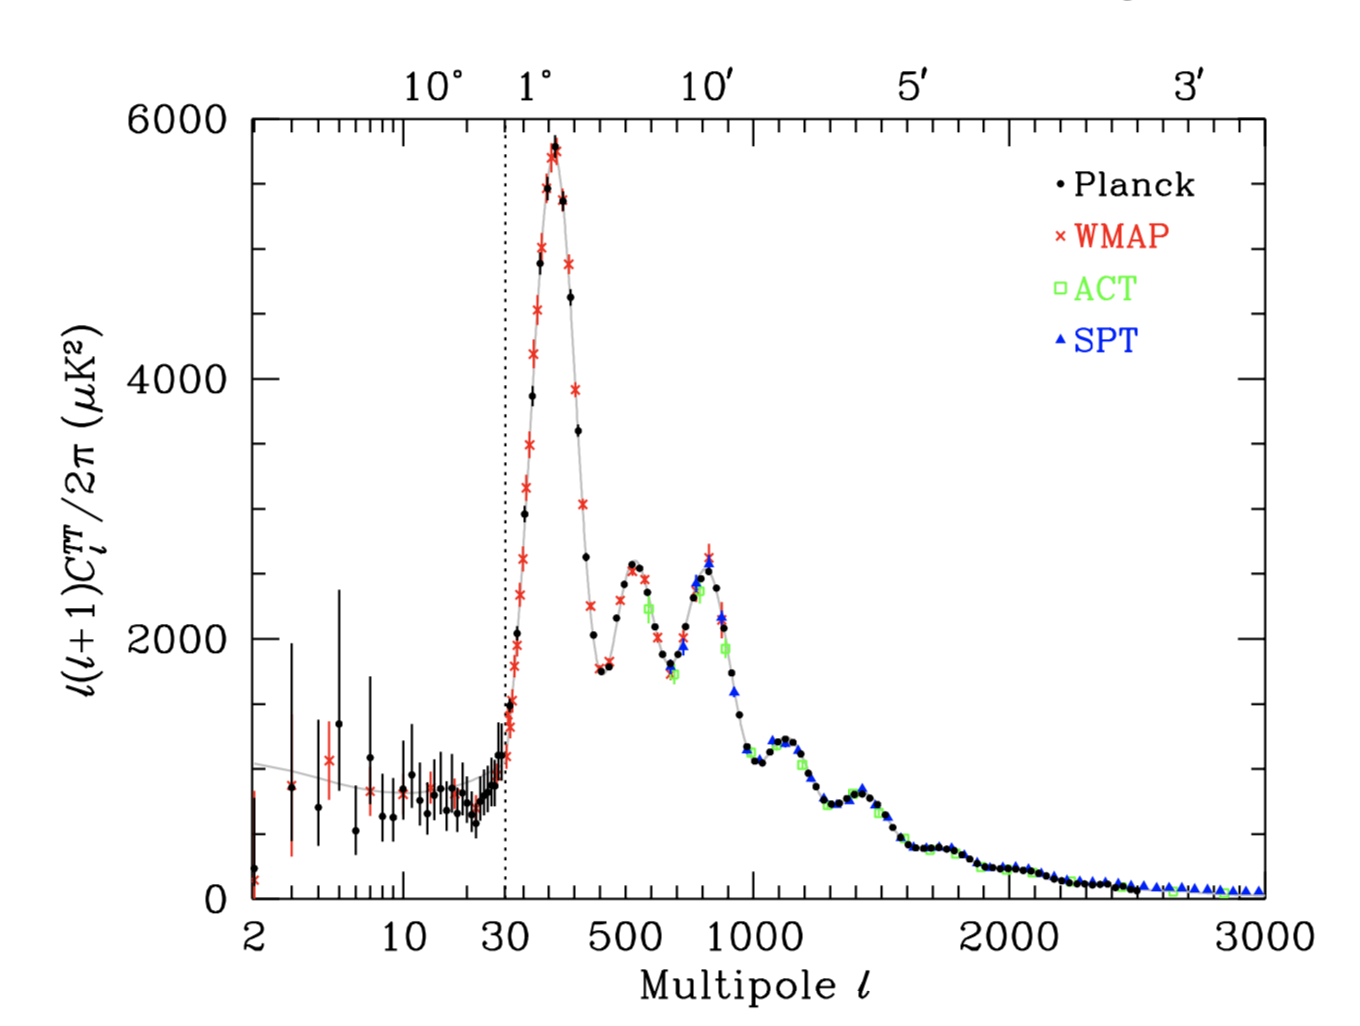
\includegraphics[width=0.8\textwidth]{figs/CMB_multipole}
  \caption{The CMB radiation temperature anisotropy power spectrum as a function of the multipole order,$\ell$, as measured by various experiments~\cite{Agashe:2014kda}. The angular scales that correspond to the multipole orders are listed across the top of the graph. The data points correspond to the experimental measurements and the error bars account for measurement uncertainties. The black curve represents the best global fit of the standard model of cosmology to the Planck data.}
  \label{fig:CMB}
\end{figure}

%In addtion, the numerical simulations  The observation that star ages within galaxies are on the order of 10 to 14 billion years old, and cluster formation is still under way serves to support the cold dark matter (CDM) hypothesis. In this case, DM comprises of rather massive, slow moving, and non-relativistic particles, which would stimulate the clumping of matter into small regions initially, eventually giving rise to larger scale structures. This bottom-up theory of structure formation is further supported by myriad computer simulations consisting of billions of dark matter particles confirming the CDM model yields large structures such as those observed by the Sloan Digital Sky Survey. 

\section{The Standard Model}
\label{sec:SM}

In the pursuit of a suitable candidate for what comprises close to $24\%$ of the total matter in the Universe, a segue to the fundamental underpinnings of the SM of particle physics is required. In this section, an overview of the SM is presented along with its most successful predictions of experimentally observed particle physics phenomena and its greatest deficiencies in the quest to explain the nature of DM. 

As a framework that describes the fundamental constituents of observed matter and their corresponding interactions, in this respect the SM is deemed exceedingly successful. Not only are such observations predicted accurately by the SM, but its organization of the fundamental building blocks of our Universe within a framework can be thought of as analagous to the organization of elements within Mendeleev's periodic table~\cite{PhysRevD.86.010001}. In the theory of the SM, three of the four fundamental forces are responsible for particle matter interactions: the electromagnetic, weak, and strong forces. A few of the matter particles which these forces act upon include protons, neutrons, electrons, and quarks, whose properties are described in detail later in this section. An example of particle interactions described by the SM is the binding of neutrons and protons via the strong force in the atomic nucleus. By contrast, the weak force is responsible for the process of a neutron decaying to a proton, during which one type of quark is transmuted to another (nuclear $\beta$ decay). The electromagnetic (EM) force is responsible for such phenomena as Bremsstrahlung, the process of EM radiation as a result of the deceleration of a charged particle deflected off another charged particle. 

The foundations of the SM began with the unification of the weak and electromagentic forces in the Glashow-Weinberg-Salam (GWS) theory of electroweak (EW) interactions~\cite{Glashow:1959wxa, Salam:1968rm, PhysRevLett.19.1264} leading to the theory of quantum electrodynamics (QED), and making the first firm prediction of mass possible~\cite{Griffiths:111880}. The strong force is described by what constitutes as the remainder of the SM, the theory of quantum chromodynamics (QCD)~\cite{PhysRevLett.30.1346,PhysRevLett.30.1343}. The remaining of the four fundamental forces, gravity, does not have a place within the SM as of yet, as it is a quantum theory used to describe the ``micro'' world and is difficult to fit into the same framework as Einstein's general theory of relativity describing the ``macro'' world, where gravity plays a significant role. Acting with vastly larger strengths over significantly shorter ranges, the EW and strong forces render the effects of gravity negligible in the context of particle physics phenomena. 

The elementary matter components of the SM are particles obeying Fermi-Dirac statistics called \textit{fermions} and have half-integer spins, while the force carriers or so-called ``messenger'' particles obey Bose-Einstein statistics, known as \textit{bosons} have integer spin. Individual fermion particle states can interact via the strong force to form \textit{baryons} such as the proton and the neutron, which consist of three \textit{quarks} (the elementary fermion particles comprising the substructure of the nucleon). Similarly, a \textit{meson} is a bosonic two-fermion bound state consisting of a quark and anti-quark pair. Any particles, whether composite like baryons or mesons, or elementary like the quark, which interact via the strong force are classed as \textit{hadrons}. Of course, there are also fermions like the electron and the neutrino which do not interact via the strong force, but rather via the electromagentic (EM), which are called \textit{leptons}. The elementary quarks, leptons, and bosons carry quantum numbers that dictate their interactions such as charge (Q), lepton number (L), baryon number (B), and spin. It should be noted that color charge (C), weak isospin (T$_{3}$), and hypercharge (Y) are also additional elementary particle quantum numbers that characterize the symmetry groups comprising the SM to be introduced later. The leptons and quarks listed in the first six rows of Table~\ref{tab:SM} are divided into three generations where a mass hierarchy is established with increase in generation. Despite the increase in mass with generation, the lifetime in general decreases, although $c$ and $b$ quarks are an exception to this trend, providing an experimental handle for their discrimination in high energy experiments. In addition, quarks and leptons of higher generations can decay to quarks and leptons of the corresponding first generation. The bottom five rows in Table~\ref{tab:SM} list the weak force carrying bosons, W and Z, the strong force carrying boson, g, the EM force carrying boson, $\gamma$, and the Higgs boson, H, which gives the other particles mass.  

\begin{table}[!htbp]
  \scalebox{0.85}{
    \begin{tabular}{l l l c c c l}
      \hline
      & Particle & Particle &      & Electric    & Mass  & Force\\
      Generation & Symbol   & Name     & Spin & Charge      & [GeV] & Interaction/Carrier \\
      \hline
      1st        & $e^-$    & Electron          & 1/2  & -1  & $5.11\times10^{-4}$ & EM, Weak \\
      & $\nu_{e}$& Electron Neutrino & 1/2  & 0   &  -                  & Weak \\
      \hline   
      2nd        & $\mu^-$     & Muon          & 1/2  & -1 & 0.106        & EM, Weak \\
      & $\nu_{\mu}$ & Muon Neutrino & 1/2  & 0  &  -           & Weak \\
      \hline
      3rd        & $\tau^-$     & Tau          & 1/2  & -1 & 1.78        & EM, Weak \\
               & $\nu_{\mu}$  & Tau Neutrino & 1/2  & 0  &  -           & Weak \\
      \hline \hline
      1st        & $u$          & Up Quark   & 1/2 & 2/3      & $\approx2.3\times10^{-3}$ & EM, Weak, Strong \\
      & $d$          & Down Quark & 1/2 & -1/3     & $\approx4.8\times10^{-3}$ & EM, Weak, Strong \\
      \hline
      2nd        & $s$          & Strange Quark & 1/2 & -1/3  & $\approx9.5\times10^{-2}$ & EM, Weak, Strong \\
      & $c$          & Charm Quark   & 1/2 & 2/3 & 1.28                      & EM, Weak, Strong \\
      \hline
      3rd        & $b$          & Bottom Quark  & 1/2 & -1/3 & 4.2                      & EM, Weak, Strong \\
               & $t$          & Top Quark     & 1/2 & 2/3  & 172.5                    & EM, Weak, Strong \\
      \hline \hline
      -          & W$^\pm$      & W Boson       & 1   & $\pm1$ & 80.4                   & Weak \\ 
      -          & Z            & Z Boson       & 1   &    0   & 91.2                   & Weak \\
      -          & $\gamma$     & Photon        & 1   &    0   & 0                      & EM   \\
      -          & g            & Gluon         & 1   &    0   & 0                      & Strong \\
      \hline\hline
      -          & H            & Higgs Boson   & 0   &    0   & 125                    & - \\
      \hline
    \end{tabular}
  }
  \caption{The particles of the SM including the leptons ($e^-$, $\mu^-$, $\tau^-$, $\nu_{e}$, $\nu_{\mu}$, $\nu_{\tau}$), the quarks ($u$, $d$, $c$, $s$, $t$, $b$), the gauge bosons (W$^\pm$, Z, g, $\gamma$), and the scalar Higgs boson (H). The spin, charge, and mass are specified where the neutrinos are taken to be massless, and indirect measurements posit the mass eigenstates are less than 0.23 eV~\cite{PhysRevD.86.010001}. The forces via which the particles interact are listed for each lepton and quark and the force mediated is listed for the gauge bosons.}
  \label{tab:SM}
\end{table}

The SM is defined in terms of a quantum field theory (QFT) Lagrangian density that adheres to certain symmetries. Just as the classical field theory of electricity and magnetism, as fully described by Maxwell's equations, remains unchanged under position, rotation, reflection, and Lorentz transformations, so the SM remains invariant under certain transformations, better known as symmetries. In the case of Maxwell's equations, when invariance under the standard translational, rotational, and reflectional symmetries are combined with invariance under Lorentz symmetry, the combined group of symmetries is termed the Poincar$\acute{\mathrm{e}}$ Lie group. The Poincar$\acute{\mathrm{e}}$ symmetry is a global (spacetime) symmetry, whereas the Lie groups of the symmetries associated with the SM are local transformations associated with fields rather than particles defined by space and time coordinates. The local or internal symmetries which are the starting point for the various parts of the SM Lagrangian, are also known as gauge symmetries. The interactions within the SM are described by specific interaction terms which modify the Lagrangian leaving it invariant under the gauge transformations. Hence, the SM is defined as a gauge QFT based on the $SU(3)_{C}\otimes SU(2)_{L}\otimes U(1)_{Y}$ symmetry groups, where the elementary particle interactions dictated by the strong force are described by the $SU(3)_{C}$ Lie group, and interactions dictated by the electroweak forces are described by $SU(2)_{L}\otimes U(1)_{Y}$.

\subsection{Electroweak theory and the Higgs mechanism}
\label{subsec:EWKHiggs}

The point of departure for the description of interactions in the SM is the Dirac Lagrangian density,

\begin{equation}
  \mathcal{L}_{D} = \bar{\psi}(i\gamma^\mu\partial_\mu - m)\psi,
  \label{eq:dirac}
\end{equation}

where $\gamma^\mu$ are the Dirac $\gamma$-matrices, $\bar{\psi} = \gamma^{0}\psi$ is the conjugate fermion field, and $m$ is the fermion mass. Defining the interactions between a two spin-$\frac{1}{2}$ fields, which can be re-written as the doublet, 

\begin{equation}
  \Psi := 
  \begin{pmatrix}
    \psi_{1} \\
    \psi_{2}
    \end{pmatrix},
  \label{eq:doublet}
\end{equation}

requires a locally $SU(2)$ invariant Lagrangian achieved through the addition of the extra term $i\bar{\Psi}\gamma_\mu \frac{\sigma_i}{2} W^\mu_i \Psi$ which describes the interactions between two spin-$\frac{1}{2}$ and three massive spin-1 fields $W^\mu_i$. This process exploits a local internal symmetry of $W^\mu_i$ where $W^\mu_i \rightarrow W^{'\mu}_i = W^\mu_i + \partial^\mu a_i(x)$. Neglecting the mass terms, the Lagrangian then reads,

\begin{equation}
  \mathcal{L}_{D1+D2+int} = i\bar{\Psi}\gamma_\mu\partial^\mu\Psi + \bar{\Psi}\gamma_\mu \frac{\sigma_i}{2} W^\mu_i \Psi,
  \label{eq:partialQED}
\end{equation}

but \EquationRef{eq:partialQED} is missing the term for the three free spin-1 fields which includes the internal symmetry as described above. When this term is added, \EquationRef{eq:partialQED} turns into,

\begin{equation}
  \mathcal{L}_{SU(2)} = i\bar{\Psi}\gamma_\mu\partial^\mu\Psi + \bar{\Psi}\gamma_\mu \frac{\sigma_i}{2} W^\mu_i \Psi - \frac{1}{4}(W_{\mu\nu})_{j}(W^{\mu\nu})_{j},
  \label{eq:SU2}
\end{equation}

with $(W_{\mu\nu})_i = \partial_\mu(W_\nu)_i  - \partial_\nu(W_\mu)_i$, and leading to an $SU(2)$ invariant Lagrangian. \EquationRef{eq:SU2} is nonetheless lacking mass terms because the introduction of terms such as $m_{1}\bar{\Psi}{\Psi}$ or $m_{2}(W^\mu)_i(W_\mu)_i$ would destroy the $SU(2)$ symmetry. Acquiring the mass terms will be done through the breaking of this symmetry by the addition of a spin-0 field. Before this however, it is possible to unify the locally $SU(2)$ invariant Lagrangian in \EquationRef{eq:SU2} with a locally $U(1)$ invariant Lagrangian in order to additionally describe fermion EM interactions. Hence, the spin-1 field $B^\mu$, also known as the $U(1)$ gauge field, is introduced where its locally $U(1)$ invariant Lagrangian goes as,

\begin{equation}
  \mathcal{L}_{U(1)} = -m\bar{\psi}\psi + \bar{\psi}\gamma_\mu(i\partial^\mu + gB^\mu)\psi - \frac{1}{4}B_{\mu\nu}B^{\mu\nu}
  \label{eq:U1}
\end{equation} 

where $B^{\mu\nu} := \partial^\mu B^\nu - \partial^\nu B^\mu$. Combining \EquationRef{eq:SU2} and \EquationRef{eq:U1} then yields the $SU(2)$ and $U(1)$ locally invariant Lagrangian,

\begin{equation}
  \mathcal{L}_{SU(2)\otimes U(1)} = \bar{\Psi}\gamma_\mu(i\partial^\mu + gB^\mu + g'\sigma_i W^\mu_i)\Psi - \frac{1}{4}(W_{\mu\nu})_{j}(W^{\mu\nu})_{j}-\frac{1}{4}B_{\mu\nu}B^{\mu\nu},
  \label{eq:SU2cU1}
\end{equation}

where the coupling constant for the three $W^\mu_i$ fields is ignored and simply denoted by $g'$. As mentioned earlier, the mass terms cannot be added ``by hand'' to the Lagrangian since they effectively spoil the symmetry, but by writing a locally $SU(2)$ invariant Lagrangian for doublets of spin-0 fields, just as done in \EquationRef{eq:partialQED} earlier for spin-$\frac{1}{2}$ fields, it will be shown how the mass terms for the $W^\mu_i$ and $B^\mu_i$ fields are attained. Thus for the spin-0 doublet $\Phi := \begin{pmatrix} \phi_1 \\ \phi_2 \end{pmatrix}$, \EquationRef{eq:SU2cU1} turns into,

\begin{equation}
  \begin{aligned}
  \mathcal{L}_{SU(2)\otimes U(1)} = ((\partial_\mu - ig'\sigma_i(W_\mu)_i - i\frac{1}{2}gB_\mu)\Phi^{\dagger})((\partial^\mu - ig'\sigma_i(W^\mu)_i + i\frac{1}{2}gB^\mu)\Phi) \\
  + \rho^2\Phi^\dagger\Phi - \lambda(\Phi^\dagger\Phi)^2,
  \end{aligned}
\label{eq:b4symbreak}
\end{equation}

where the last two terms on the right-hand side are defined collectively as $-V(\Phi)$, or are better known as the Higgs potential. $V(\Phi)$ can in fact be written as a function of one of the spin-0 doublet fields, $V(\phi)$, so that the minimum of $V(\phi) = -\rho^2|\phi|^2 + \lambda|\phi|^4$ can be computed in the traditional way by $\frac{\partial V(\phi)}{\partial\phi} = 0$. This leads to a minimum $\phi_{\mathrm{min}} = \sqrt{\frac{\rho^2}{2\lambda}}e^{i\phi}$ meaning that for every $\phi$ value there exists a minimum and thus there are an infinite number of minima, all of which lie on a circle with radius $\sqrt{\frac{\rho^2}{2\lambda}}$. Best visualized by the 3-dimensional $V(\phi)$ function in the complex plane in ~\FigureRef{fig:mexhat}, a minimum is chosen out of the infinite possibilities (i.e. symmetry breaking), in the same sense that a marble would roll down from the top of the ``sombrero'' potential and spontaneously or randomly choose a vacuum value to settle in, out of infinite possibilities. 

\begin{figure}
  \centering
  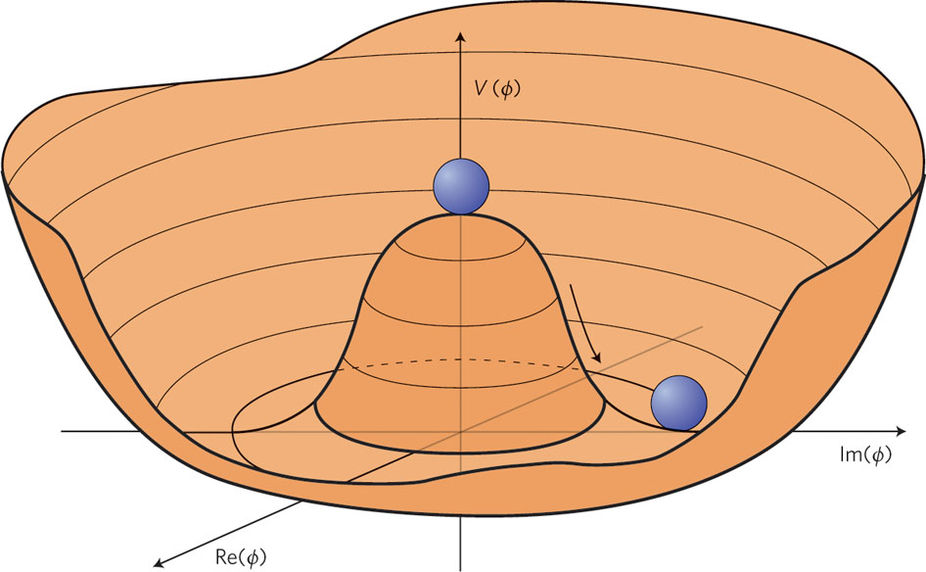
\includegraphics[width=0.7\textwidth]{figs/mexhat}
  \caption{The vacuum value, or the lowest-energy state, of the Higgs potential as shown in the 3-dimensional plot is described by a randomly chosen point at the bottom of the ``sombrero''~\cite{Alvarez-Gaume:2010aa}.}
  \label{fig:mexhat}
\end{figure}

The spin-0 doublet can then be re-written as,

\begin{equation}
  \Phi_{\mathrm{min}} = \begin{pmatrix} 0 \\ \sqrt{\frac{\rho^2}{2\lambda}} \end{pmatrix} \equiv \begin{pmatrix} 0 \\ \frac{v}{\sqrt{2}} \end{pmatrix},
  \label{eq:higgsdoublet}
\end{equation}

where the redefinition of the minimum in terms of $v$ is chosen for brevity. Substituting the field $\Phi$ with the minimum shifted field in what is known as the unitary gauge, $\Phi_{\mathrm{min}}$, and subsequently performing the matrix algebra of the first term in \EquationRef{eq:b4symbreak}, the following expression is attained,

\begin{equation}
  \frac{v^2}{8}(g')^2((W^\mu_1)^2 + (W^\mu_2)^2) + (g'W^\mu_3 - gB^\mu)^2),
  \label{eq:massbreak}
\end{equation} 

where two new spin-1 fields can be defined from the old ones,

\begin{equation}
  W^\mu_{+} \equiv \frac{1}{\sqrt{2}}(W^\mu_1 -iW^\mu_2) \\
  W^\mu_{-} \equiv \frac{1}{\sqrt{2}}(W^\mu_1 +iW^\mu_2),
\end{equation}

where $W^\mu_{+}$ and $W^\mu_{-}$ are complex conjugates of one another, and the first term in \EquationRef{eq:massbreak} becomes $\frac{1}{8}v^2g'^{2}(W^+)_\mu(W^-)^\mu$. At last, the W boson mass term ($\frac{1}{2}M_{W}^2 = \frac{1}{8}v^2g'^{2}$) is given! Similarly, the second term in \EquationRef{eq:massbreak} can be expanded with matrix diagonalization, and the remaining spin-1 fields, $W^\mu_3$ and $B^\mu$, can be interpreted in terms of the new spin-1 fields, 

\begin{equation}
  Z_\mu = W^\mu_3\cos{\theta_W} - B^\mu\sin{\theta_W}, \\
  A^\mu = W^\mu_3\sin{\theta_W} + B^\mu\cos{\theta_W},
\end{equation} 

where $\theta_W$ is the weak mixing angle (or Weinberg angle), and is given by $\tan^{-1}(\frac{g'}{g})$ and the terms in \EquationRef{eq:massbreak} become,

\begin{equation}
  \frac{1}{8}v^2g'^{2}(W^+)_\mu(W^-)^\mu + \frac{1}{8}v^2\frac{g'^{2}}{\cos{\theta_W}^2}Z_\mu^2 + \frac{1}{8}v^2\cdot0\cdot A_\mu^2.
  \label{eq:EWmass}
\end{equation}

The fields can then be identified with the bosons in Table~\ref{tab:SM} where $A_\mu$ is the photon. The masses of the fields can be read off as,

\begin{equation}
  \begin{split}
    & M_W = \frac{g'v}{2} \\ 
    & M_Z = \frac{g'v}{2\cos{\theta_W}} = \frac{M_W}{\cos{\theta_W}} \\ 
    & M_A = 0 
  \end{split}
\end{equation}

Hence, the Higgs mechanism is the means by which the gauge theory of massless bosons, after symmetry breaking, becomes a theory of masssive bosons. In addition, the Higgs field vacuum expectation value, $v$ is 246 GeV. From the steps above which lead to the field responsible for the Z boson $Z_\mu$ and the field responsible for the photon $A_\mu$, it can be seen that both have a common point of departure, since they are orthogonal linear combinations of the fields $B_\mu$ and $W_\mu^3$. 

\subsection{Yukawa interactions}
\label{subsec:yukawa}

In addition to allowing bosons to have mass, the Higgs mechanism gives fermions their masses without destroying gauge invariance after symmetry breaking. This is a particularly attractive feature of the SM, since the same Higgs doublet that generates the $W^\pm$ and Z masses suffices to allow for lepton and quark masses. In order to ensure that gauge invariance is retained, the new interaction terms in the Lagrangian between the spin-$\frac{1}{2}$ fields and the spin-0 Higgs field with the doublet as $\Phi := \frac{1}{\sqrt{2}}\begin{pmatrix} 0 \\ v + h \end{pmatrix}$, where h describes a physical Higgs boson, is

\begin{equation}
  \mathcal{L}_{Hf\bar{f}} = -(h_d)_{ij}\bar{q}_{L_i}\Phi d_{R_j} - (h_u)_{ij}\bar{q}_{L_i}(-i\sigma_2\Phi^*)u_{R_j} - (h_\ell)_{ij}\bar{\ell}_{L_i}\Phi \ell_{R_j}.
  \label{eq:fermioncoupling}
\end{equation}

From this, it can be seen that the Higgs couples to quark doublets, which are left chiral states (L) under $SU(2)$ transformations, and to either up or down-type right chiral (R) quark singlets (i.e. $u_{R}$ and $d_{R}$). The Higgs doublet also has couplings to left-handed lepton doublets and charged right-handed lepton singlets. Once the $SU(2)\otimes U(1)$ symmetry is spontaneously broken then \EquationRef{eq:fermioncoupling} becomes,

\begin{equation}
  \mathcal{L}_{m_f} = (m_d)_{ij}\bar{d}_{L_i}d_{R_j} + (m_u)_{ij}\bar{u}_{L_i}u_{R_j} + (m_e)_{ij}\bar{e}_{L_i}e_{R_j},
  \label{eq:fermionmass}
\end{equation}

where $m_{f} = \frac{y_{f}v}{\sqrt{2}}$, with $y_f$ being the Yukawa coupling for a fermion $f$. $u_L$, $d_L$, and $e_L$ are the up-type quark, down-type quark and lepton doublet components defined as,

\begin{equation}
\begin{split}
&  \begin{pmatrix} 
    u \\
    d'
  \end{pmatrix}_L
  \begin{pmatrix} 
    c \\
    s'
  \end{pmatrix}_L
  \begin{pmatrix} 
    t \\
    b'
  \end{pmatrix}_L
  \\
&  \begin{pmatrix} 
    \nu_e \\
    e
  \end{pmatrix}_L
  \begin{pmatrix} 
    \nu_\mu \\
    \mu
  \end{pmatrix}_L
  \begin{pmatrix} 
    \nu_\tau \\
    \tau
  \end{pmatrix}_L
\end{split}
\end{equation}

Thus, the relation between the fermion mass and the Yukawa coupling demonstrates that heavier fermions correspond to fields that are more strongly coupled to the Higgs boson. In order to go from the quark weak eigenstates ($d'$, $s'$, $b'$) to the corresponding mass eigenstates, the Cabbibo-Kobayashi-Maskawa (CKM) matrix below is used,

\begin{equation}
  \begin{pmatrix}
    d' \\
    s' \\
    b'
  \end{pmatrix} 
  =
  \begin{pmatrix}
    V_{ud} & V_{us} & V_{ub} \\
    V_{cd} & V_{cs} & V_{cb} \\
    V_{td} & V_{ts} & V_{tb}
  \end{pmatrix}
  \begin{pmatrix}
    d \\
    s \\
    b
  \end{pmatrix}
  \label{eq:CKM}
\end{equation} 

where the CKM matrix values are, 

\begin{equation}
  \begin{pmatrix}
    V_{ud} & V_{us} & V_{ub} \\
    V_{cd} & V_{cs} & V_{cb} \\
    V_{td} & V_{ts} & V_{tb}
  \end{pmatrix}
 = 
\begin{pmatrix}
  0.974 & 0.225 & 0.004 \\
  0.225 & 0.973 & 0.041 \\ 
  0.009 & 0.040 & 0.999
\end{pmatrix}
\end{equation}

It can be noted that the CKM matrix is nearly the identity, thus transitions between fermion generations are heavily suppressed, but by contrast a top quark decays to a W boson and b quark at a rate of $99.9\%$. Quark couplings to the W boson are in part characterized by the CKM matrix in what follows as the Lagrangian for charged currents,

\begin{equation}
  \mathcal{L}_{\mathrm{CC}} = \frac{g}{\sqrt{2}}W_\mu^+(\nu_L \gamma^\mu e_L + V_{\mathrm{CKM}}\bar{u}_L\gamma^\mu d_L) + \frac{g}{\sqrt{2}}W_\mu^-(\bar{e}_L\gamma^\mu\nu_L + V_{\mathrm{CKM}}\bar{d}_L\gamma^\mu u_L),
\end{equation}

where $u$ denotes up-type quarks, $d$ denotes down-type quarks, $\nu$ denotes neutrinos, and $e$ denotes charged leptons. From the subscript, it can be noted that only left-handed fermions (and right-handed antifermions) couple to the W$^\pm$, hence there is a 100$\%$ breaking of parity ($\mathcal{P}$) and charge conjugation ($\mathcal{C}$), however gauge invariance is still preserved under the combined $\mathcal{CP}$ symmetry. Similarly, quarks and leptons couple to the neutral carriers of electroweak interactions, the Z boson and the photon, via the neutral current Lagrangian given by,

\begin{equation}
  \mathcal{L}_{\mathrm{NC}} = \sum_{j}\bar{\psi}_j \gamma^\mu\ \Big\{ A_\mu [g \frac{\sigma_3}{2}\sin\theta_W + g'y_j \cos\theta_W] + Z_\mu[g\frac{\sigma_3}{2}\cos\theta_W - g'y_j\sin\theta_W] \Big\}\psi_j,
\end{equation}

where for simplicity we take,

\begin{equation} 
  \psi_1 = \begin{pmatrix} u \\ d \end{pmatrix}_L, \:\:\: \psi_2 = u_R, \:\:\: \psi_3 = d_R,\:\mathrm{or} \\
  \psi_1 = \begin{pmatrix} \nu_e \\ e^- \end{pmatrix}_L, \:\:\: \psi_2 = {\nu_e}_R, \:\:\: \psi_3 = {e^-}_R.
\end{equation}

The EM coupling is defined as $e = g\sin\theta_W = g'\cos\theta_W$ and a relation between the fermion hypercharge ($Y$), electric charge ($Q$) and weak isospin ($T_3$) quantum numbers can be established with $T_3 \equiv \sigma_3/2$ and $Y = Q - T_3$. Hence, for quarks and leptons,

\begin{equation}
  \mathrm{Quarks:}\: y_1 = Q_u - \frac{1}{2} = Q_d + \frac{1}{2} = \frac{1}{6},\:\:\:\:\: y_2 = Q_u = \frac{2}{3}, \:\:\:\:\: y_3 = Q_d = -\frac{1}{3}, \\
  \mathrm{Leptons:}\: y_1 = Q_\nu - \frac{1}{2} = Q_e + \frac{1}{2} = -\frac{1}{2},\:\:\:\:\: y_2 = Q_\nu = 0, \:\:\:\:\: y_3 = Q_e = -1.
\end{equation}

Thus, it is shown that fermions with the same electric charge have the same universal couplings, and neutrinos do not have EM interactions ($Q_\nu=0$) although their coupling to the W and Z boson is non-zero. Examining the properties of the neutrino more closely, one might be tempted to propose it as a viable DM particle candidate since it satisfies \textit{some} of the key requirements for a suitable candidate, those being:

\begin{itemize}
  \item Stability on the order of the cosmic timescale, as required to remain in existence currently
  \item No strong or EM interactions
  \item Non-baryonic, since the potential baryon fraction of DM is known to be small
  \item Combined with any other DM particles/constituents, the total DM must have the correct relic density
\end{itemize}

It will however, become clear in the following section, why the neutrino, as predicted by the SM, is an insufficient contender for $24\%$ of the matter fraction in the Universe. Analogously, the SM, as briefly described in this section, successfully predicts observed particle physics phenomena to a high degree of accuracy, with the most recent experimental confirmation being the discovery of a $125\:\GeV$ particle compatible with the predicted Higgs boson, by the ATLAS and CMS experiments at the LHC in 2012~\cite{Aad:2012tfa,Chatrchyan:2012xdj}. Nonetheless, there exist a number of theoretical and phenomenological problems, which cannot be accommodated by the SM. Among those are the hierarchy problem, wherein the Planck scale ($M_{Pl} \sim 10^{18}\:\GeV$), the point at which gravity is as strong as the gauge interactions, is nearly $\mathcal{O}(10^{15})$ larger than the electroweak scale, both of which are widely considered fundamental energy scales in nature. In addition, the matter-antimatter asymmetry that exists in the Universe today does not jive with the SM prediction that approximately equal amounts of matter and antimatter should have been created during the earliest phases of the Universe, had a proportionate amount of matter compared to antimatter existed during the initial conditions. Other open issues such as the addition of small, but nonetheless experimentally observed neutrino mass~\cite{Feldman:2013vca} to the SM is not possible unless other key free parameters are modified which leads to further theoretical complications of the SM framework. Alongside these open questions is the lack of a fundamental particle candidate supplied by the SM to explain the vast amount of DM in as observed in the Universe. Possible extensions to the SM can help to alleviate the tension presented between the above physical phenomena and the to-date widely accepted model, where the hints of BSM physics would manifest as experimental observations of deviations from SM processes.

\section{Dark matter candidates}
\label{sec:DMcandidates}

Returning to the example of a neutrino as a possible particle DM candidate can help to elucidate the properties which have lead to the most dominant model, currently. During the early stages of the Universe, when the rate of cosmic expansion overtook the rate at which weak interactions in equilibrium proceeded, such as neutron-proton conversion given by $n \leftrightarrow p + e^- + \bar{\nu}_e$, the process of SM neutrino decoupling from the background radiation occured. At this so-called ``freeze out'' stage, the neutrino is relativistic and remains as such during the later stages of galaxy and larger structure formation, owing also to its near massless nature. Relativistic particles moving throughout the Universe, however, are generators of high pressure, which cause a smoothening and subsequent destruction of any small matter density fluctuations and would ultimately not lead to the large scale structure formation as observed today. Evidence from N-body simulations made as early as 1983 by White, Frenk, and Davis~\cite{White:1984yj} present a vastly inconsistent picture of galaxy clustering than what is observed, and consequently definitively rule out a neutrino-dominated Universe.

The SM neutrino is part of a larger classification of particle DM, known as hot dark matter (HDM). HDM candidates are very light particles with $m_{\mathrm{HDM}} < 1\:\mathrm{eV}$, and are typically disfavored as leading candidates since they hinder large scale structure formation as a result of their relativistic energies. Although HDM certainly exists in our Universe today, such as SM neutrinos, current observational data place an upper limit of $0.25\%$ of the fraction of mass in the Universe as contributed by HDM. On the other hand, at the other end of the energy spectrum are DM candidates which are non-relativistic at the time of decoupling from the thermal bath, and are classed as cold dark matter (CDM). With a mass ranging between $\mathcal{O}(\GeV) < m_\mathrm{CDM} < \mathcal{O}(\TeV)$, the lower velocities of CDM in contrast to those of HDM would result in a short range dispersion with respect to the size of the Universe, and generate very little pressure, allowing for the clustering of stars and galaxies to form the filaments and structures observed today. Numerous N-body simulations commencing from random density fields of non-interacting CDM demonstrate these observations~\cite{10.1093}. Situated between HDM and CDM, warm dark matter (WDM), is postulated to have $m_{\mathrm{WDM}} \simeq \mathcal{O}(\mathrm{keV})$. Although relativistic at the time of decoupling, WDM then cools during the radiation-to-matter transition phase and becomes non-relativistic causing some smoothening of dense knots of matter, but still allowing for structure formation. Sterile neutrinos, gravitinos, and photinos fall under this category, but WDM is disfavored in large part because N-body simulations are less consistent with observations than those for CDM candidates.

The leading DM candidate, which is classified as a type of CDM, is the weakly interacting massive particle (WIMP) and to-date it is the most theoretically desirable candidate for a number of reasons. One of the strongest arguments for a WIMP as a DM candidate, should it exist and be stable, is that the relic density it would produce is consistent with that required by DM. The mechanism via which this occurs is referred to as the ``WIMP miracle'', alluding to the notion that WIMPs, although originally proposed as a solution to the gauge hierarchy problem, are extremely suitable DM candidates as well. As mentioned earlier, the thermal freeze-out period of the Universe occured when interactions with the thermal bath which reach an equilibrium can no longer keep up with the rate of expansion of the Universe, hence after freeze-out, interactions which affect the total number of WIMPs are negligible. The exchange of energy between SM particles and WIMPs may still proceed efficiently, however. Quantitatively, the number density of the DM particle, $n$, can be described by the Boltzmann equation,

\begin{equation}
  \frac{dn}{dt} = -3Hn - \langle\sigma_A v \rangle(n^2 - n_{\mathrm{eq}}^2),
  \label{eq:boltz}
\end{equation}

where H is the Hubble constant, $\langle\sigma_A v\rangle$ is the thermally averaged annihilation cross section and $n_{\mathrm{eq}}$ is the DM number density in thermal equilibrium. In order to obtain the thermal relic density, \EquationRef{eq:boltz} is solved numerically, where the freeze-out time is defined as $n\langle\sigma_{A} v\rangle = H$ and leads to~\cite{PhysRevD.33.1585},
\begin{equation}
  \Omega_{\chi} \simeq \frac{\mDM T_0^3}{\rho_c M_{Pl} T_f} (\langle \sigma_A v \rangle)^{-1},
\label{eq:Omega}
\end{equation}
where $\rho_c$ denotes the critical density, $\mDM$ denotes the DM mass, and $T_0$ and $T_f$ denote the present and freeze-out time temperatures. It can be noted that $\Omega_{\chi}$ has an inversely proportional relationship to the velocity-averaged annihilation cross section and does not strongly depend on the mass of the DM. Thus, for WIMPs postulated to be in the $\mathcal{O}(\GeV) < \mDM < \mathcal{O}(\TeV)$ mass range, assuming that the annihilation cross section into SM particles is on the order of the electroweak scale, the observed $\Omega_{\chi}$ is correctly predicted by the WIMP miracle, as visualized in~\FigureRef{fig:WIMPrelic}.

\begin{figure}
  \centering
  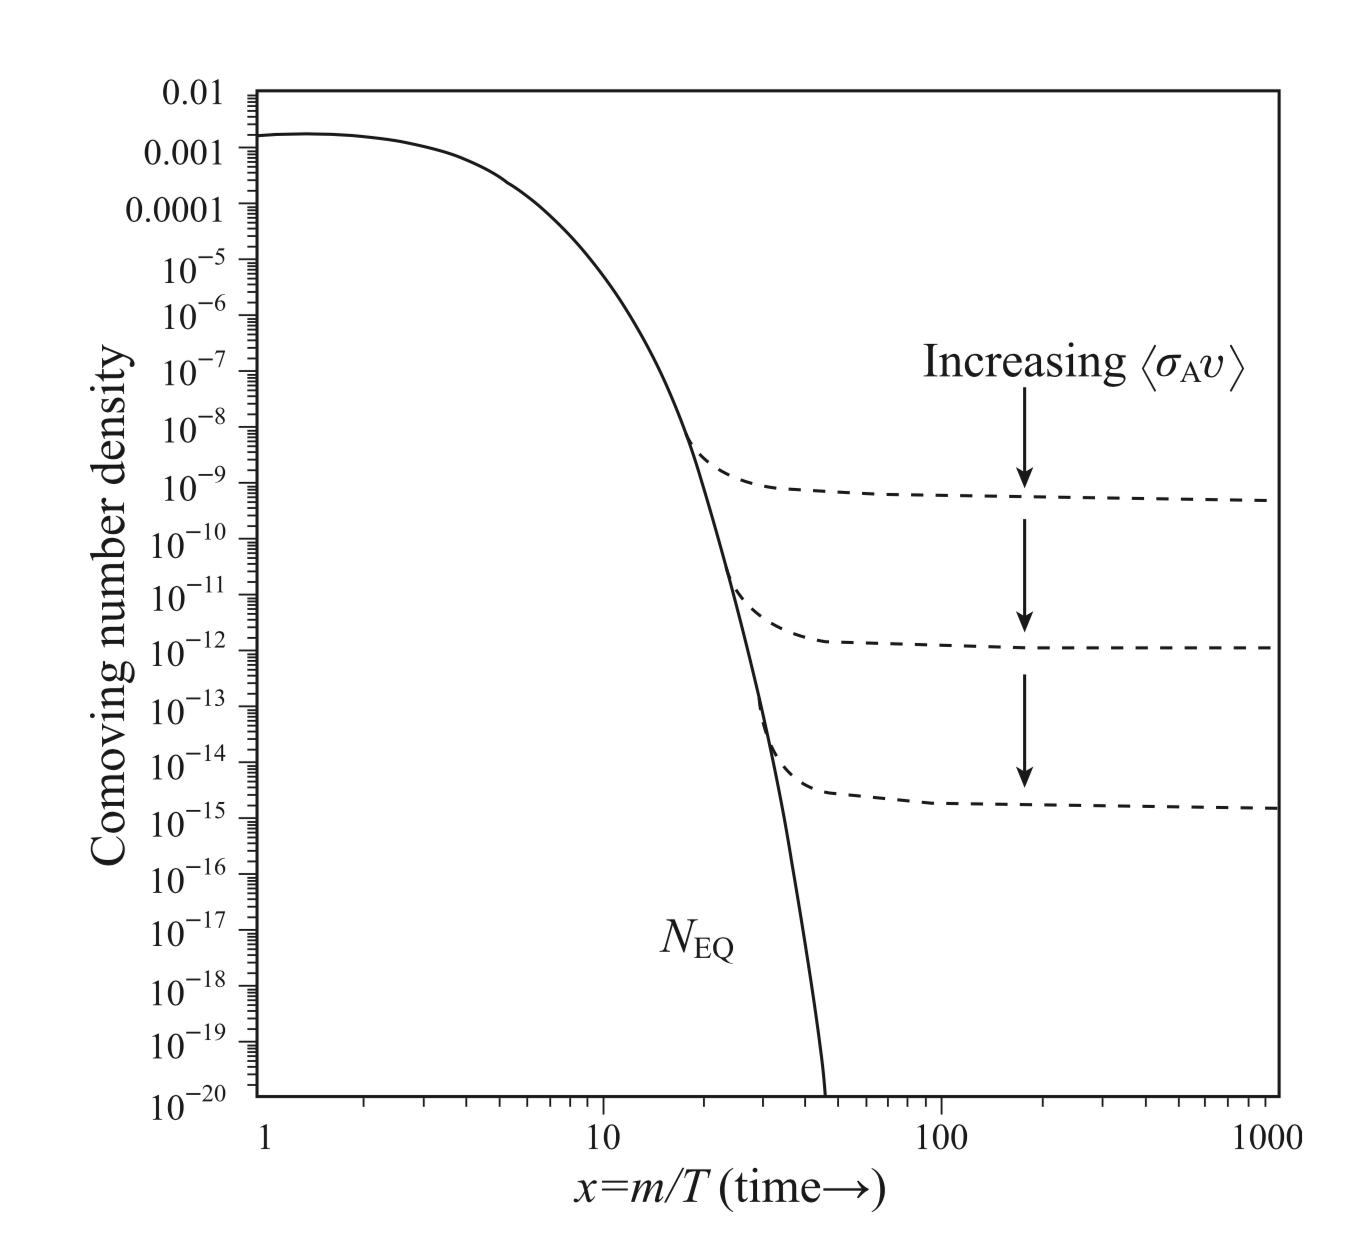
\includegraphics[width=0.6\textwidth]{figs/WIMP_thermal_relic}
  \caption{The WIMP comoving number density as a function of time, also parametrized as $x_f = \frac{\mDM}{T_f}$, where an increase in the annihilation cross section ultimately results in a later freeze-out time, and a correspondingly lower thermal relic density~\cite{Kolb:1990vq}.}
  \label{fig:WIMPrelic}
\end{figure}

Thus, yielding a naturally correct $\Omega_\chi$ via the freeze-out production mechanism, and characterized by the kinematic qualities of CDM which predict the structure formation observed in the Universe today, the WIMP is the most theoretically preferred DM candidate. WIMPs are predicted by many BSM theories, whether as neutralinos in supersymmetric (SUSY) theories, super-heavy and super-weakly-interacting particles coupling to SM fields via the Higgs portal called WIMPzillas, or through effective field theory operators (EFT) which describe the weak contact interaction between SM particles and DM. In short, the WIMP provides model-independent grounds for weak scale DM production, which furthermore allows the experimental community to search for its existence via multiple independent and complementary methods.

\section{Dark matter detection}
\label{sec:DMsearches}

Favorable implications for DM detection arise as a result of the WIMP miracle. In order to reach the correct relic density, the WIMP DM particles must also annhilate to other particles, which are assumed to be SM particles. The process of $\chi \bar{\chi} \rightarrow \mathrm{SM}\:\mathrm{SM}$ means it is possible to write down the elastic scattering and annihilation cross sections of DM and ordinary particles within a framework of a particle physics theory. It has been established that DM is responsible in part for the dynamics of galaxies and clusters, which in turn lead to the large scale structures observed today. The galactic halo of our own Milky Way galaxy is predicted to be abundantly filled with DM particles, and the WIMP model would allow for the detection of signals emitted by DM annihilation to SM particles. Conversely, the stability and proliferation of WIMPs would allow DM particles to reach terrestrial laboratories, where a potential DM signal would reveal itself as elastic scattering of DM off ordinary particles depositing energy in sensitive detectors. By construction, the WIMP paradigm would also allow for the reversal of the annihiliation process, such that the production of pairs of DM particles from extremely highly energetic SM particles is possible. The annihilation, elastic scattering, and production of DM are the underlying strategies respectively used by indirect, direct, and collider methods of DM detection detailed in this section.

\subsection{Indirect detection}
\label{subsec:ID}

Although DM makes up a substantial part of the Universe, it nonetheless, does not constitute the entirety of the energy-mass density ratio, thus the observed $\Omega_\chi$ was reached through its annihilation. The WIMP miracle implies that DM-SM interactions must be efficient, thus if DM annihilation occured during the early Universe, it must also proceed in the same way today albeit at a lower frequency, making it possible to detect the SM products from the reaction. Indirect searches for DM target a large region of the cosmos, such as the sun, the galactic halo of the Milky Way and that of other galaxies. An indirect detection (ID) signal would typically manifest itself as an anomalous event of cosmic rays, where DM annihilation results in an abnormally high rate of SM particle-anti-particle pair production. Fluxes of cosmic rays can encompass a large number of particles though most ID experiments focus on signatures of charged particles ($e^- e^+$, $p \bar{p}$, deuterium and antideuterium), photons (in the form of gamma rays, X-rays, or synchrotron radiation), and lastly, neutrinos. Experiments dedicated to searches of charged anti-particle fluxes make good use of the under-abundance of anti-particles with respect to their corresponding particles in the Universe, whereas dedicated photon and neutrino flux experiments target areas of the cosmos that can maximize the potential DM signal to noise from astrophysical sources. The cosmic fluxes of the aforementioned elementary particles are a result of the showering and hadronization of the pair-produced primary particles from the DM annihilation, such as $b\bar{b}$, $\mu^+\mu^-$, $\tau^+\tau^-$, and $W^+W^-$. The spectra of the cosmic rays depends in large part on the mass of the primary particles that emmitted the flux, but in general the distribution features a 'bump'-like structure which is characterized by a high-energy cutoff at the \mDM. 

\begin{figure}
  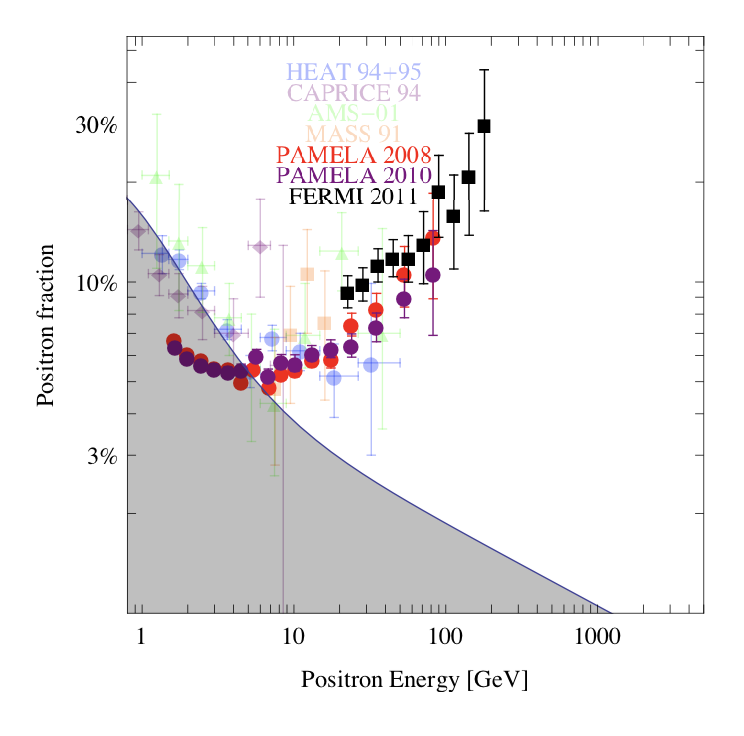
\includegraphics[width=0.7\textwidth]{figs/pamela.png}
  \caption{The positron energy spectra measured by a compilation of recent (PAMELA and FERMI) and less recent ID experiments dedicated to measurements of secondary charged particles emmitted in cosmic ray fluxes. The data is superimposed on a compilation of uncertain astrophysical backgrounds from secondary production.~\cite{Cirelli:2012tf}}
  \label{fig:positronflux}
\end{figure}

Myriad ID experiments are currently under operation or are projected for future searches. An example of one such experiment is the PAMELA satellite~\cite{Adriani:2008zr} which presented an excess over a potential but uncertain background from secondary astrophysical sources in the positron energy spectra for $10\:\GeV < E_{e^+} < 100\:\GeV$, as seen in~\FigureRef{fig:positronflux}. The excess was also extended to $200\:\GeV$ and confirmed independently by measurements from the FERMI satellite~\cite{PhysRevLett.108.011103}, and the prototype Alpha Magnetic Spectromenter (AMS-01) experiment~\cite{Aguilar:2007yf}. Although the signals seem quite striking since it implies a source of $e^+$ exists other than ordinary astrophysical ones, it is precisely the uncertainties in these backgrounds and their potentially exotic contributions to the spectra that limit the interpretation of ID signals as DM. In this respect, not only are other ID experiments necessary to confirm a signal as a potential DM discovery, but another means of detection altogether is required to corroborate a signal from indirect detection methods, since improving the simulation and understanding of astrophysical backgrounds is non-trivial.

\subsection{Direct detection}
\label{subsec:DD}

The non-relativistic nature of the WIMP would allow for its detection via elastic scattering off a SM particle, which imparts a transfer of momentum to the nucleus, known as the nuclear recoil. Direct detection (DD) experiments are sensitive to the secondary effect of the nuclear recoil and thus detect a potential WIMP signature through the light, heat, or ionization of the SM material with which it interacted. DD experiments are typically conducted in deep, underground terrestrial laboratories in order to suppress the highly energized neutron fluxes produced from cosmic rays that penetrate the atmosphere, since such backgrounds are the most serious and challenging to disentangle from a potential signal. A sufficient amount of Earth material or water/ice is necessary to shield the highly sensitive detectors and reduce the high cosmic muon intensity fluxes. Furthermore, as a result of the small interaction rate of DM-SM particles, DD experiments observe single interactions as opposed to multiple interactions, and it thus follows that any interactions would be uniformly distributed within the detector volume, contrasting the background from radioactivity expected at the detector surface.

The formalism of WIMP DD is summarized in the following steps, where more details are given in \cite{Jungman:1995df}:

\begin{itemize}
\item The kinetic energy of a recoiled nucleus, after elastic scattering is approximately,

\begin{equation}
  E_{r} \approx (\frac{1}{2}\mDM v^2)\Big(\frac{4\mDM m_N}{(\mDM + m_N)^2}\Big)\cos^2{\theta_R},
  \label{eq:kinE}
\end{equation}

where $\theta_R$ is the angle of nuclear recoil, $m_N$ is the mass of the nucleus, and $v$ is the velocity of $\chi$ relative to the detector in question. With an expected WIMP local density in the Milky Way galactic halo of $\rho_{\chi 0}=0.4\:\GeV/c^2/cm^3$, $v^2$ is approximately $\mathcal{O}(10^{-6})$ at the average detector depth, and \EquationRef{eq:kinE} is maximized to a value of $10^{-6}\mDM$ when the DM and nucleus mass are equal. Thus a WIMP mass on the order of $100\:\GeV$ would lead to $E_r \approx 0-100\:\mathrm{keV}$.

\item The detection rate depends on the reaction cross section of the DM and the SM nucleus collision, which can be parametrized as a function of the nuclear momentum transfer $q_r = 2m_rv\cos\theta_r$, where $m_r$ is the reduced mass of the $\chi-N$ system. The parametrization leads to a differential cross section of a recoiled nucleus,

\begin{equation}
  \frac{\mathrm{d}\sigma(q_r)}{\mathrm{d} q_r^2} = \frac{\sigma_0}{(2m_r v)^2}F^2(q_r),
\label{eq:diffxsec}
\end{equation}

where the denominator on the right-hand side of \EquationRef{eq:diffxsec} is the square of the maximal momentum transfer that occurs for forward scattering. The form factor, $F(q_r)$, accounts for the finite size of the nucleus and can depend on whether the DM-SM interaction is spin-independent (SI) or spin-dependent (SD). In addition, the total recoil cross section, $\sigma_0$, has SI and SD contributions, where the $\sigma_{SI}$ depends on the couplings of the WIMP to protons and neutrons in the given model, though generically they are expected to be equal.

\item The interaction rate per unit detector mass in a given velocity range $[v,v+dv]$ goes as,

\begin{equation}
  dR = \Big(\frac{\rho_{\chi 0}}{m_\chi m_N}\Big) v \frac{\mathrm{d}\sigma(q_r)}{\mathrm{d} q_r^2} f_1(v)\mathrm{d}v\mathrm{d}q_r^2
\label{eq:DDrate}
\end{equation}

where the $f_1(v)$ is a Maxwellian distribution that models the galactic WIMP velocity. 

\item The velocity integration in \EquationRef{eq:DDrate} gives the rate as a function of the recoil energy from \EquationRef{eq:kinE} and yields,

\begin{equation}
  \frac{dR}{dE_r} \propto \exp{\Big(\frac{-m_N E_r}{2m_r^2v_0^2}\Big)}.
\end{equation}

Thus, in contrast to the expected peak structure that would be observed by ID experiments, the recoil spectrum that DD experiments look for is approximately described by an exponential. For this reason, there is no precise spectral signature, and most of the signal is expected to lie at the low recoil energy range requiring a firm understanding of the experimental energy thresholds of dedicated WIMP direct detectors.
\end{itemize}

Unlike ID experiments, DD experiments may make some assumption on the particle physics model which dictates the values of $\sigma_0$ and $F(q_r)$ ultimately changing the interaction rate expected in a given type of detector material. Taking the example of a neutralino ($\tilde{\chi}^0$) from SUSY models as the WIMP candidate, the $\tilde{\chi}^0$-nucleon cross section depends on the coupling between the $\tilde{\chi}^0$ and quarks in the low-energy regime. These interactions are mediated through scalar, pseudoscalar, axial, and axial-vector currents, in the same manner that electroweak interactions are mediated via gauge $vector$ bosons. In particular, the $\tilde{\chi}^0$ is a Majorana fermion~\cite{Majorana2006}, and thus can only couple to the particles in the SM sector via scalar or axial-vector currents. Axial-vector and pseudoscalar couplings give rise to SD WIMP-nucleon cross sections, while vector and scalar couplings generate SI cross sections.

The most sensitive SI DD searches make use of low-temperature heat and ionization detectors, or consist of dual-phase noble liquids. Since the SI cross section is directly proportional to the target nucleus mass, such detectors employ heavy nuclei such as xenon (Xe) and germanium (Ge). An example of one such experiment is the XENON1T experiment~\cite{refId0}, which makes use of liquid Xe (LXe) time projection chambers (TPCs). Located at a depth of 3600 m at the INFN Laboratori Nazionali del Gran Sasso (LNGS), 2 t of ultra-pure LXe serves as the active target material in the detector which produces prompt scintillation (S1) once a particle is incident upon the target LXe nucleus. Secondary electron ionization is also produced from the energy deposit and once the electrons pass through the drift field, they are extracted into gaseous Xe (GXe) where they produce proportional scintillation light (S2). The XENON1T experiment utilizes the ratio S2/S1 to discriminate between nuclear recoils produced by WIMP or neutron interactions and electronic recoil from $\beta$ or $\gamma$ interactions. The results from the XENON1T experiment improve upon the those from PandaX-II~\cite{PhysRevLett.119.181302} and LUX~\cite{PhysRevLett.118.021303}, both technologically similar experiments. As shown in~\FigureRef{fig:xenon1t}, the recent XENON1T results exclude WIMP-nucleon $\sigma_{SI}$ of $\mathcal{O}(10^{-46})\:\mathrm{cm}^2$ for $\mDM \approx 20-30\:\GeV$, and demonstrate a seven-fold improvement in sensitivity over PandaX-II and LUX for $\mDM > 50\:\GeV$ as seen in the inset by the limits normalized to the median of the XENON1T sensitivity. Over the past several decades, the detector volume of DD experiments has expanded with the aim of increasing the sensitivity by maximal exposure. The XENON1T experiment is projected to be superceded by XENONnT, an 8 t detector predicted to reach a $\sigma_{SI}$ limit of $1.6\times10^{-48}\:\mathrm{cm}^2$ for $\mDM\approx 50\:\GeV$~\cite{2017APS..APR.J9003A}.

\begin{figure}
  \centering
  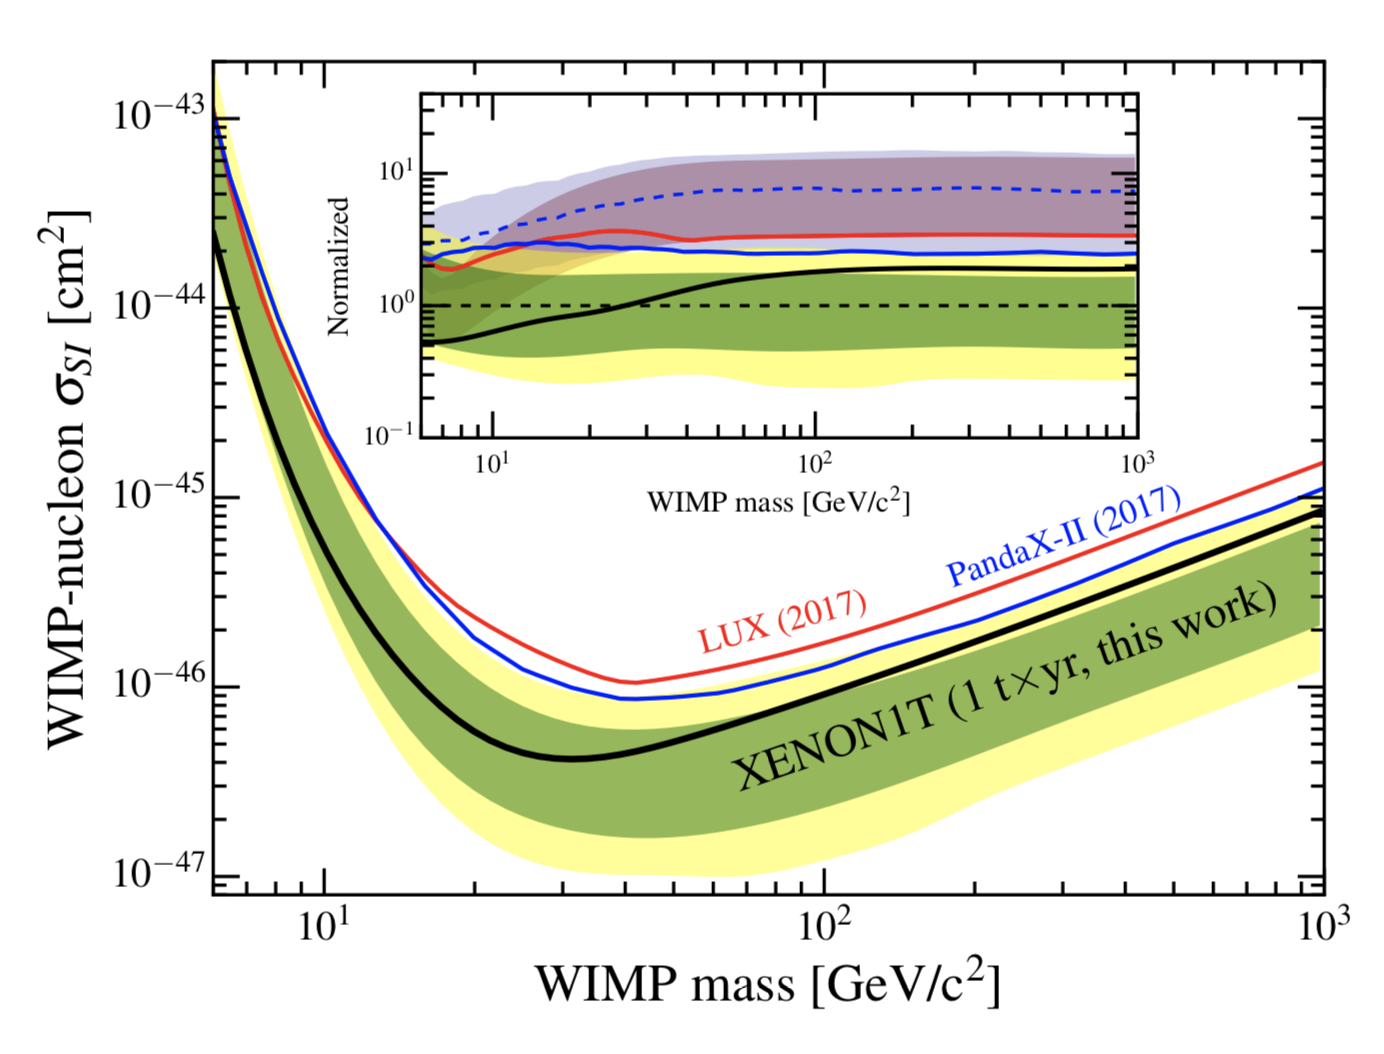
\includegraphics[width=0.7\textwidth]{figs/Xenon1T}
  \caption{Cross section limits as a function of the DM mass for spin-independent interactions for PandaX-II, LUX, and XENON1T.}
  \label{fig:xenon1t}
\end{figure}

The SD DD experiments are instead strongly reliant on the spin content of the target nucleus, and essentially translate to a constraint on the WIMP coupling coefficients to protons, $a_p$, or neutrons, $a_n$ which affect the form factor in \EquationRef{eq:diffxsec}. These experiments can also employ dual-phase noble gas TPCs, or solid scintillators and superheated bubble chambers to achieve high sensitivities at high and low \mDM, respectively. At present, the strongest constraints to SD WIMP-proton interactions are given by thermodynamically operated superheated detectors containing fluorine-rich liquids. Filled with approximately 52 kg of $\mathrm{C}_3\mathrm{F}_8$ target and operated at SNOLAB in Sudbury, Canada, the PICO-60 bubble chamber sets the most stringent constraints on the WIMP-proton $\sigma_{SD}$ at $3.4\times 10^{-41} \mathrm{cm}^2$ for $\mDM=30\:\GeV$~\cite{Amole:2017dex}.
 
\subsection{Collider searches}
\label{subsec:Collider}

As is the case with direct DM detection, searches for DM production at colliders also take into account the possible particle nature of DM, allowing in many cases for a comparison between these two vastly differing search strategies. In order to emulate the high temperature environment of the early Universe during which WIMPs are postulated to have been produced, the energy of the colliding SM particles at accelerators is necessarily very high. The accelerated particles are typically extremely light, such as protons, anti-protons, electrons or positrons, allowing for their collision energy to be maximized. As a result, collider searches are particularly sensitive to very low WIMP masses on $\mathcal{O}(\GeV)$. However, if DM is much heavier than the $\mathcal{O}(\TeV)$ scale, it may be the case that the center-of-mass energy available at present collider experiments is insufficient to kinematically allow for the production of DM. Even if DM is produced promptly within the detecting volume at a collider, the further complication for these searches is the lack of experimental signature. DM particles would not interact with the detector material and only reveal their presence through an imbalance of total transverse momentum, also known as missing transverse energy (\MET). This quantity, described in detail in \SectionRef{sec:MET}, can be understood as the application of the laws of conservation of energy and conservation of momentum to a collision to infer the presence of a weakly interacting particles. SM neutrinos manifest as \MET in a detector because of their extremely weak interactions with the material. The saving grace of collider searches is that SM particles are predicted to be produced in conjunction with the DM particles by a plethora of relevant particle physics models. The experimental feasibilty is therefore increased for such searches, since the differential distributions of SM background processes are sufficiently well-understood, that even minute deviations from the expected \MET spectrum would allow for the constraint of DM models predicting such signals. The following section will explore the physics model context in which WIMPs are produced and collider searches are interpreted by this work.

\section{Simplified models of DM: beyond the Standard Model}
\label{sec:BSM}

As mentioned earlier, the production of DM within different types of BSM particle physics models probed by collider searches allows for the detection of a potential signal indirectly via the SM particles that are expected to be produced in association with the WIMPs. Such searches performed by the ATLAS and CMS collaborations are termed $\text{Mono}$-$X$ searches, where the $X$ is the SM particle(s) produced together with the DM particles. The models which the searches in question target, are numerous and span a range of completeness. Supersymmetric (SUSY) extensions to the SM are amongst the most complete BSM theories, and correspondingly incur the largest number of model parameters. SUSY models also do not necessarily directly tie together the annhilation of SM particles to the production of DM particles, since the DM particles are often secondarily produced together with a significant number of SM particles. The constraints that exist for SUSY models are also, in large part, not related to the DM particle itself, but apply to a greater degree to the other parameters. In favor of a simpler description of the DM-SM interactions, a class of models characterized by fewer tuneable parameters, albeit less theoretically complete, are investigated in this work. 

DM production at colliders can be described, in large part, by the interaction between the SM and DM particles. Prior to Run II of the LHC, DM searches such as the one detailed in~\cite{Khachatryan:2016reg}, had been traditionally interpreted using Effective Field Theory (EFT) models~\cite{Goodman:2010ku}, wherein the interaction between the SM particles and the Dirac fermion WIMPs is mediated through higher dimensional operators. The models are solely characterized by \mDM, and $M_{*}$ which represents the strength of the interaction and is a function of the masses and coupling strengths of the mediating particles between the DM and SM fields. The benefit of the EFT formulation is the lesser degree of model dependence, and the relative ease encountered in translating experimental collider constraints to the direct detection DM-nucleon cross section-\mDM plane. The shortcoming of such field theories, however, are that they are non-renormalizable, thus they become invalid at arbitrarily high energy scales. This is represented by the masses of the mediating particles that have been integrated out. In general, for an EFT to make sense, it is required that $M_{*}$ be much larger than the energy transfer through quarks at the LHC, $M_{*}^{2} \gg Q_{\textrm{tr}}^{2}$. Put another way, the EFT formalism is valid only if the energy scale of the interaction involving the DM and the SM particles is small with respect to the energy scale associated to the heavy mediator, $M_{*}$. In general, ID and DD experiments adhere to this requirement since the expected energy transfers are of the order of \mDM or $\mathcal{O}(\mathrm{keV})$, respectively. In the high energy environment of collider searches, however, the processes that might be described by the EFT operators would occur in a region beyond the validity of the theory~\cite{BUSONI2014412}. Thus, since this class of models does not truly account for the mediator, effects from resonant enhancement are not included and EFTs have no description of off-shell mediator production.

In order to circumvent the deficiencies of the EFT formalism, a class of \textit{simplified models} have been employed for the interpretation of DM searches during Run II of the LHC. In part, the increase in the center-of-mass collision energy from $\sqrt{s}=8\:\TeV$ to $\sqrt{s}=13\:\TeV$ further limits the region of validity for the EFT models. Hence, the contact interaction of the EFT models, as depicted in~\FigureRef{subfig:EFT}, is subsequently resolved into a mediator interaction which couples to the SM and DM particles, as shown in~\FigureRef{subfig:DMsimp}, thus increasing the free parameters to include the coupling of the mediator to the SM sector, \gq, the coupling of the mediator to the DM sector, \gDM, the mass of the mediator, \mMed, and \mDM. For comparison,~\FigureRef{subfig:SUSY} shows a SUSY model of sgluon-mediated ($\tilde{g}$), di-squark ($\tilde{q}$) decay to SM particles and $\tilde{\chi}^0$s.\FigureRef{subfig:DMsimp} is called a simplified model of DM and in particular, the Feynman diagram represents a spin-1 s-channel mediated process where at least one SM particle from initial state radiation and a $\chi\bar{\chi}$ pair is expected.

\begin{figure}
  \subfloat[][EFT model]{\label{subfig:EFT} 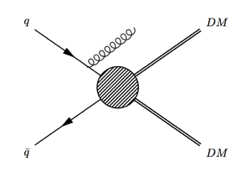
\includegraphics[width=0.3\textwidth]{figs/MJ_EFT}}
  \subfloat[][Simplified model of DM]{\label{subfig:DMsimp} 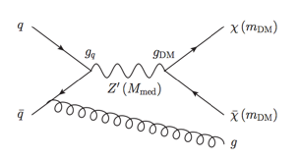
\includegraphics[width=0.3\textwidth]{figs/MJ_DMSimp}}
  \subfloat[][SUSY model]{\label{subfig:SUSY} 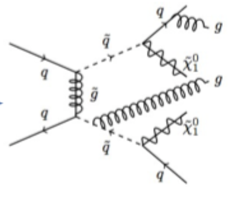
\includegraphics[width=0.3\textwidth]{figs/SUSY}}
\caption{}
\label{fig:models}
\end{figure}

Simplified DM models are built upon three major criteria:

\begin{itemize}
  \item The DM particle must be absolutely stable or else have a lifetime long enough to escape the LHC detectors
  \item The Lagrangian should contain renormalizable terms which are also Lorentz invariant, obey the SM gauge symmetries and give stable DM
  \item Additional interactions between the DM and SM sector must conserve baryon and lepton number and only break custodial and flavor symmetries softly~\cite{Abdallah:2015ter}
\end{itemize}

The third criterion is met by the assumption of Minimal Flavor Violation (MFV)~\cite{PhysRevLett.65.2939} which curbs flavor and $\mathcal{CP}$-violation in models of new physics. The essential idea behind MFV is that new physics must preserve the general structure of flavor-changing neutral current (FCNC) processes present in the SM. Thus, any flavor and $\mathcal{CP}$-violating transitions are entirely dictated by the CKM matrix. In particular, this work is focused on the minimally flavor violating spin-0 models, where it is shown in \cite{Abdallah:2015ter} that through MFV the $s$-channel couplings of the SM fermions to the DM sector are required to be of Yukawa type. The interaction Lagrangians of the spin-0 scalar ($\phi$) and pseudoscalar ($a$) mediators are as follows~\cite{Abercrombie:2015wmb},

\begin{equation}
  \mathcal{L}_{\phi} = g_{\chi}\phi\chi\bar{\chi} + \frac{\phi}{\sqrt{2}}\sum_{i}{(g_{u}y_{i}^{u}\bar{u}_{i}u_{i} + g_{d}y_{i}^{d}\bar{d}_{i}d_{i} + g_{\ell}y_{i}^{\ell}\bar{\ell}_{i}\ell_{i})},\\
  \mathcal{L}_{a} = ig_{\chi}a\chi\gamma_{5}\bar{\chi} + \frac{ia}{\sqrt{2}}\sum_{i}{(g_{u}y_{i}^{u}\bar{u}_{i}\gamma_{5}u_{i} + g_{d}y_{i}^{d}\bar{d}_{i}\gamma_{5}d_{i} + g_{\ell}y_{i}^{\ell}\bar{\ell}_{i}\gamma_{5}\ell_{i})}
\end{equation}

where the Yukawa couplings are $y_{i}^{f} = \sqrt{2}m_{i}^{f}/v$, where $m^{f}_{i}$ is the fermion mass, and $v=246\:\GeV$ is the Higgs boson field vacuum expectation value. $g_{u}, g_{d}$ and $g_{\ell}$ represent the coupling strength between the mediator and up-type quarks, down-type quarks, and leptons respectively. In the report issued by the Dark Matter Forum (DMF)~\cite{Abercrombie:2015wmb}, a collaboration between members of CMS, ATLAS and the theory community, a benchmark set of parameters for the relevant simplified models of DM were chosen after scans of the parameter space were performed. In the following work, the DMF recommendation of $\gDM = g_{u} = g_{d} = g_{\ell} = 1$ has been adopted. This reduces the free parameters to \{\mDM, \mMed\} which contribute to the minimal mediator width at leading order (LO) via, 

\begin{equation}
  \Gamma_{\phi} = \frac{\mDM}{8\pi}\Big(1-\frac{4\mDM^{2}}{m_{\phi}^2}\Big)^{x/2} + \sum_{f=fermions}\frac{y_{f}^{2}m_\phi}{16\pi}\Big(1 - \frac{4m_{f}^2}{m_{\phi}^2}\Big)^{x/2},
  \label{eq:width}
\end{equation}

with $x=3$ for scalar mediators, and $x=1$ for pseudoscalar mediators. Owing to the choice of SM Higgs-like Yukawa couplings for the SM fermions, the top quark contribution to the mediator width is enhanced at mediator masses above twice the top quark mass, but conversely for lighter mediator masses, the DM contribution dominates since couplings to the lighter quarks are Yukawa-suppressed. In addition, since the Yukawa-type coupling of the spin-0 mediator to the SM favors the more massive of the fermion generations, this strongly motivates searching for DM produced in association with heavy flavor quarks, such as top quarks. The standard EFT diagram characterizing \ttDM production is shown in~\FigureRef{fig:EFT}, while the simplified model investigated in this work can be seen in~\FigureRef{fig:DMF}.

\begin{figure}
  \subfloat[][]{\label{fig:EFT}
    \feynmandiagram[vertical=b to d]{
      a [particle=\(\bar{t}\)] -- [fermion] b -- [fermion] c -- [fermion] d -- [fermion] e [particle=\(t\)],
      f [particle=\(g\)] -- [gluon] b,
      g [particle=\(g\)] -- [gluon] d,
      h [particle=\(\bar{\chi}\)] -- [fermion] c -- [fermion] i [particle=\(\chi\)],
      h -- [opacity=0.001] i,
      %%f -- [opacity=0.001] g,
      a -- [opacity=0.001] h,
      e -- [opacity=0.001] i,
    };
  }
  \hspace{0.5cm}
  \subfloat[][]{\label{fig:DMF}
    \feynmandiagram[horizontal=c to h]{
      a [particle=\(\bar{t}\)] -- [fermion] b -- [fermion] c -- [fermion] d -- [fermion] e [particle=\(t\)],
      f [particle=\(g\)] -- [gluon] b,
      g [particle=\(g\)] -- [gluon] d,
      c -- [scalar, edge label=\(\phi \slash a\)] h,
      i [particle=\(\bar{\chi}\)] -- [fermion] h -- [fermion] j [particle=\(\chi\)],
      e -- [opacity=0.0001] i,
      a -- [opacity=0.0001] j,
      i -- [opacity=0.0001] j,
      %%      f -- [opacity=0.0001] g,
    };
  }
  \caption{The representative diagram of a top quark pair produced in association with a pair of DM particles ($\chi\bar{\chi}$) using~\protect\subref{fig:EFT} the EFT formalism and~\protect\subref{fig:DMF} the simplified model formalism.}
\end{figure}
